\begin{figure*}[!t]
\centering

% 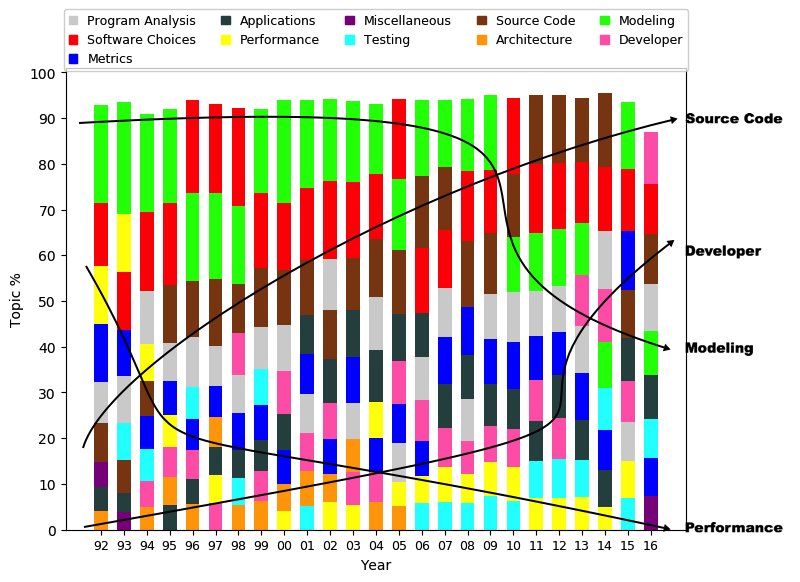
\includegraphics[scale=0.55]{figs/png_topic_evolution_all.png}
% \caption{This figure shows a stacked column chart of the contribution(in \%) of each topic in all the conferences and journals used in this study certain year between 1992-2016. The bars are stacked in ascending order;i.e. the lowest bar is most published that year and the highest bar is the least.
% }\label{fig:topic_evo_all}

{\centering 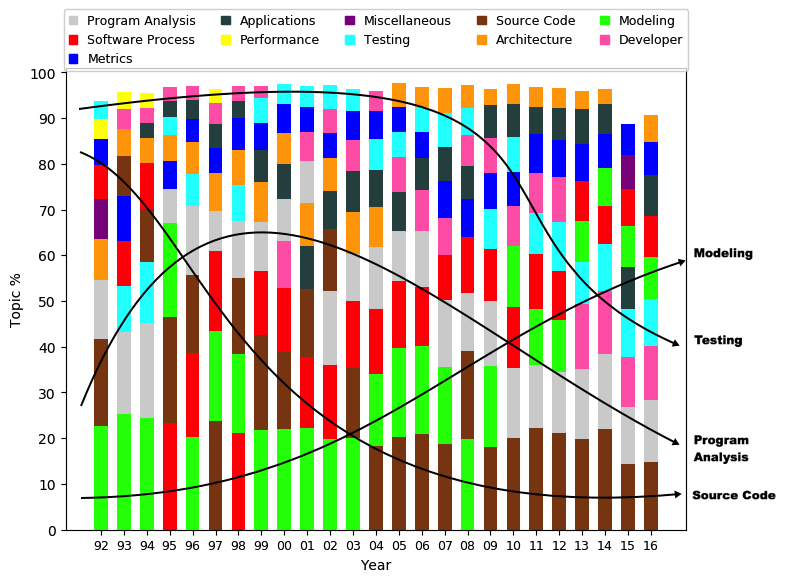
\includegraphics[scale=0.57]{png_topic_evolution_conferences.png}}
% \captionsetup{width=.8\linewidth}
\caption{Changes in {\bf conference} topics, 1992-2016.
Arrows are used to highlight the major trends.
This is a {\em stacked} diagram where, for each year, the {\em most}
popular topic appears at the {\em bottom} of each stack. That is,
as topics become {\em more} frequent, they fall towards the {\em bottom} of the plot. Conversely, as topics become {\em less} frequent,
then rise towards the {\em top}.}\label{fig:topic_evo_conferences}
 
\end{figure*}